% Edison Automation - 5-minute Beamer deck (revamped).
% Compile with:  pdflatex edison-presentation.tex
%
% Theme: metropolis if available, with a graceful fallback to Madrid so the
% deck stays portable on any reasonably complete TeX Live / MiKTeX install.
%
% 7 slides, ~40-45s each:
%   1. Title
%   2. Who I am  (with photo placeholder; drop images/partha.jpg to use a photo)
%   3. The Edison Papers project site  (edison.rutgers.edu)
%   4. The Edison Papers Digital Edition  (edisondigital.rutgers.edu)
%   5. Overall goal
%   6. Architecture
%   7. One-week MVP pipeline

\documentclass[aspectratio=169,10pt]{beamer}

\IfFileExists{beamerthememetropolis.sty}{%
  \usetheme{metropolis}%
}{%
  \usetheme{Madrid}%
  \usecolortheme{seahorse}%
}

\usepackage[T1]{fontenc}
\usepackage[utf8]{inputenc}
\usepackage{graphicx}
\usepackage{tikz}
\usepackage{xcolor}
\usepackage{hyperref}

\graphicspath{{images/}}

\definecolor{edisonAccent}{HTML}{B30838}
\definecolor{placeholderBg}{HTML}{F1F1F1}
\definecolor{placeholderFg}{HTML}{8A8A8A}

\title{Evolving the Edison Papers}
\subtitle{From Digital Archive to Research Platform}
\author{Partha Pediredla}
\institute{Rutgers University}
\date{}

\begin{document}

%% ---------------------------------------------------------------------------
%% Slide 1 - Title
%% ---------------------------------------------------------------------------
\begin{frame}[plain]
  \titlepage
\end{frame}

%% ---------------------------------------------------------------------------
%% Slide 2 - Who I am (with photo placeholder)
%% ---------------------------------------------------------------------------
\begin{frame}{Who I am}
  \begin{columns}[T,onlytextwidth]
    \begin{column}{0.35\textwidth}
      \centering
      % Drop a file at images/partha.jpg (or .png) to replace the placeholder.
      \IfFileExists{images/partha.jpg}{%
        \includegraphics[width=\linewidth,height=0.62\textheight,keepaspectratio]{partha.jpg}%
      }{\IfFileExists{images/partha.png}{%
        \includegraphics[width=\linewidth,height=0.62\textheight,keepaspectratio]{partha.png}%
      }{%
        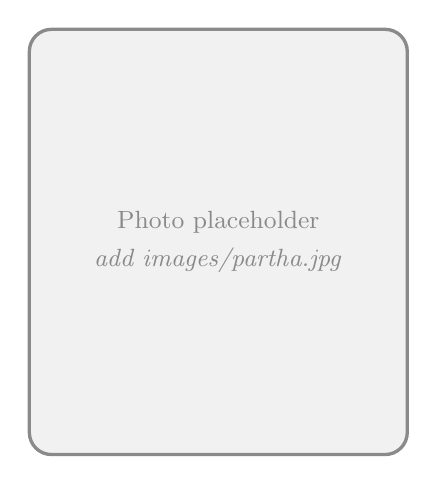
\begin{tikzpicture}
          \draw[rounded corners=8pt, very thick, draw=placeholderFg, fill=placeholderBg]
            (0,0) rectangle (4.8,5.4);
          \node[align=center, text=placeholderFg, font=\small]
            at (2.4,2.7) {Photo placeholder\\[0.3em]\textit{add images/partha.jpg}};
        \end{tikzpicture}%
      }}
    \end{column}
    \begin{column}{0.6\textwidth}
      \vspace{0.4em}
      \textbf{\large Partha Pediredla}\\[0.2em]
      {\footnotesize Rising Senior, Rutgers University}\\[1em]
      \begin{itemize}
        \setlength\itemsep{0.45em}
        \item Electrical \& Computer Engineering + Mathematics
        \item Interests: ML, AI / prompt engineering, Python, APIs
        \item Role: building the automation pipeline for the Edison Papers
      \end{itemize}
    \end{column}
  \end{columns}
\end{frame}

%% ---------------------------------------------------------------------------
%% Slide 3 - The Edison Papers project site
%% ---------------------------------------------------------------------------
\begin{frame}{The Thomas A.\ Edison Papers -- Project Site}
  \begin{columns}[T,onlytextwidth]
    \begin{column}{0.38\textwidth}
      \begin{itemize}
        \setlength\itemsep{0.55em}
        \item Rutgers' Edison Papers Project
        \item Biography, inventions, research
        \item Hosted at\\ \href{https://edison.rutgers.edu}{\texttt{edison.rutgers.edu}}
      \end{itemize}
    \end{column}
    \begin{column}{0.60\textwidth}
      \centering
      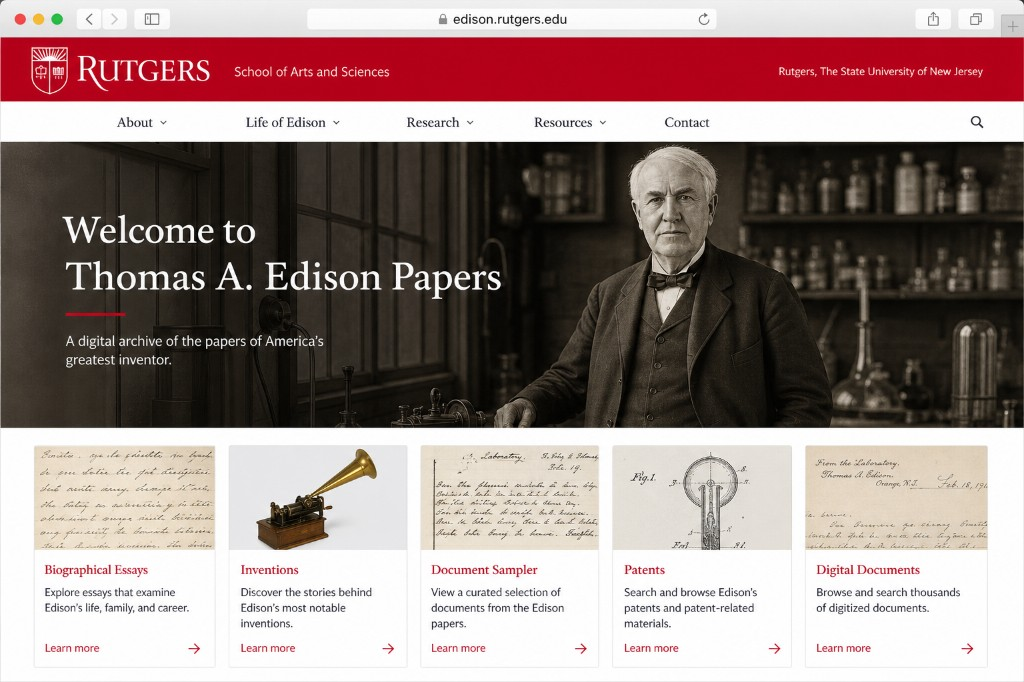
\includegraphics[width=\linewidth,height=0.78\textheight,keepaspectratio]{site-edison.png}
    \end{column}
  \end{columns}
\end{frame}

%% ---------------------------------------------------------------------------
%% Slide 4 - The Edison Papers Digital Edition
%% ---------------------------------------------------------------------------
\begin{frame}{The Thomas A.\ Edison Papers Digital Edition}
  \begin{columns}[T,onlytextwidth]
    \begin{column}{0.38\textwidth}
      \begin{itemize}
        \setlength\itemsep{0.55em}
        \item $\sim$154{,}000 digitized documents
        \item Hosted on Omeka S at\\ \href{https://edisondigital.rutgers.edu}{\texttt{edisondigital.rutgers.edu}}
        \item Works today as a digital archive:\\ browse, filter, view scanned pages
      \end{itemize}
    \end{column}
    \begin{column}{0.60\textwidth}
      \centering
      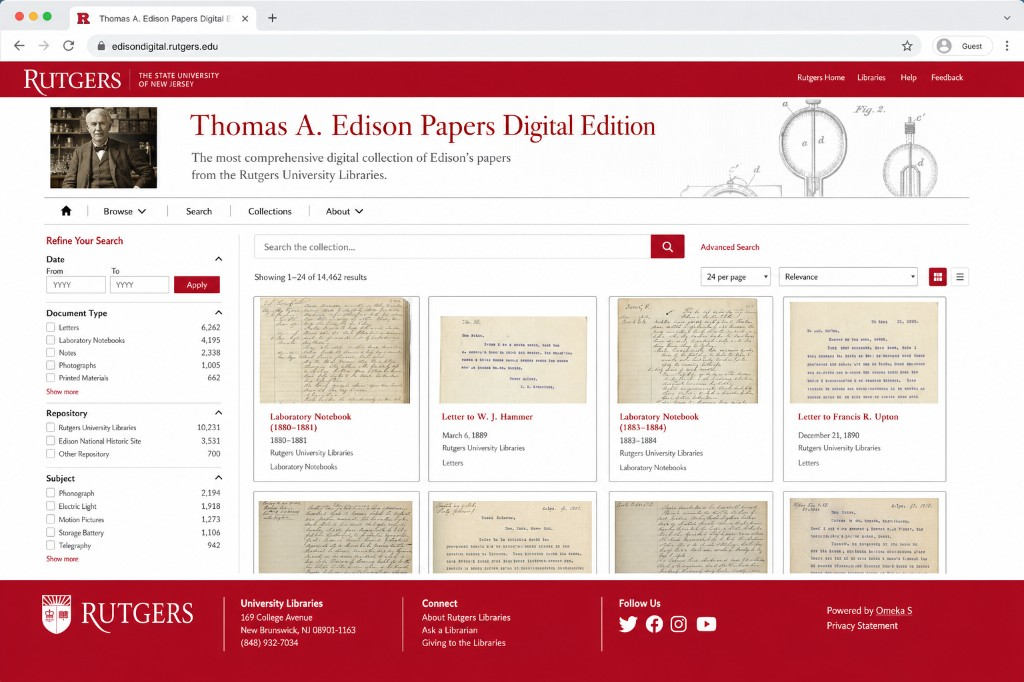
\includegraphics[width=\linewidth,height=0.78\textheight,keepaspectratio]{site-edisondigital.png}
    \end{column}
  \end{columns}
\end{frame}

%% ---------------------------------------------------------------------------
%% Slide 4 - Overall goal
%% ---------------------------------------------------------------------------
\begin{frame}{Overall goal}
  \begin{itemize}
    \setlength\itemsep{0.6em}
    \item Static archive $\rightarrow$ dynamic research platform
    \item AI transcription of all documents
    \item AI indexing for new documents
    \item Semantic search across the corpus
    \item APIs for digital humanities scholarship
  \end{itemize}
\end{frame}

%% ---------------------------------------------------------------------------
%% Slide 5 - Architecture
%% ---------------------------------------------------------------------------
\begin{frame}{Architecture}
  \begin{center}
    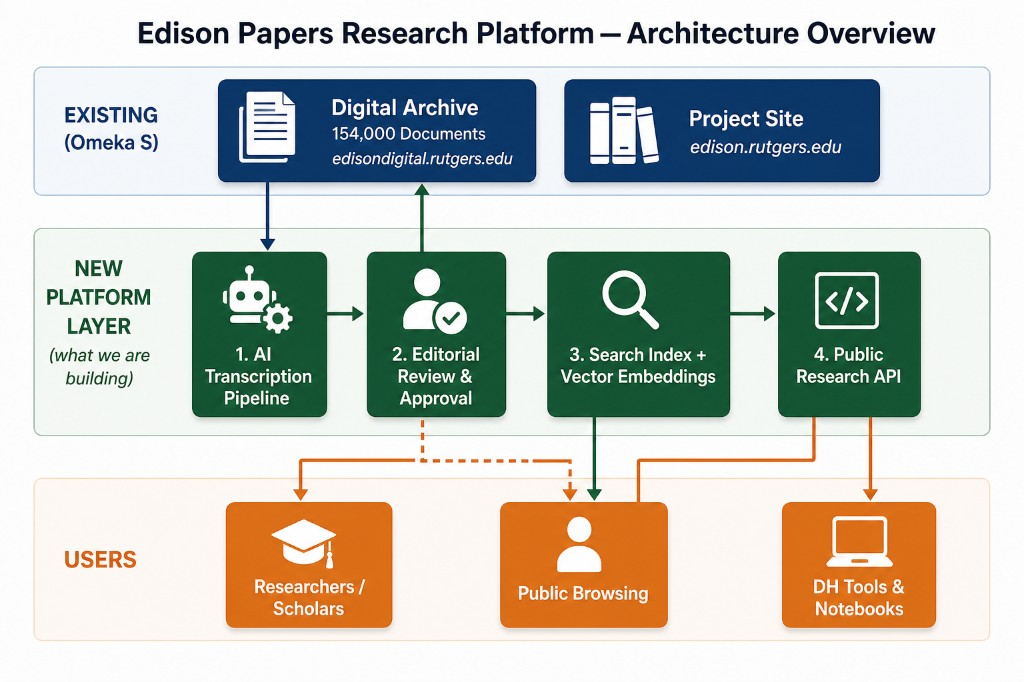
\includegraphics[width=\linewidth,height=0.82\textheight,keepaspectratio]{architecture-diagram.png}
  \end{center}
\end{frame}

%% ---------------------------------------------------------------------------
%% Slide 6 - One-week goal: MVP pipeline
%% ---------------------------------------------------------------------------
\begin{frame}{One-week goal: fundamental automation pipeline}
  \begin{center}
    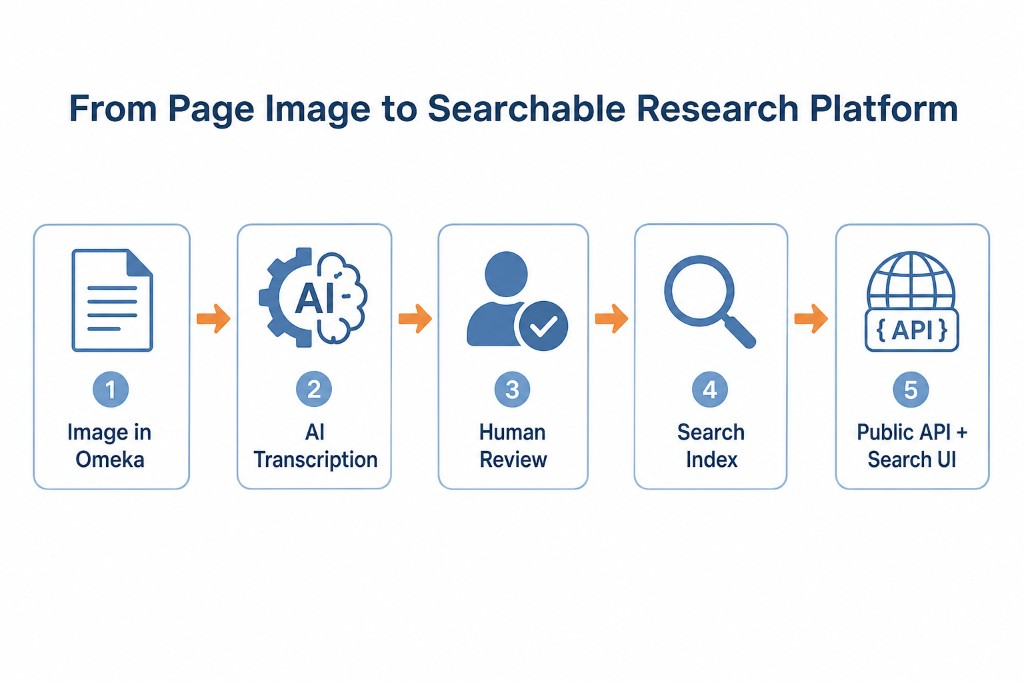
\includegraphics[width=\linewidth,height=0.72\textheight,keepaspectratio]{pipeline-flow.png}
  \end{center}
  \vspace{0.3em}
  \begin{center}
    \footnotesize Raw scans $\rightarrow$ transcribed $\rightarrow$ indexed $\rightarrow$ ready for human editing \& verification.
  \end{center}
\end{frame}

\end{document}
